\documentclass[14pt,a4paper]{report}
\usepackage[utf8]{inputenc}
%Idioma
\usepackage[spanish]{babel}
%Para expresiones matematicas
\usepackage{titlesec}
\usepackage{amsmath}
\usepackage{bm}
\usepackage{amsfonts}
\usepackage{amssymb}
\usepackage{amstext}
\usepackage{mathtools}
\usepackage{mathrsfs}
\usepackage{physics}
%Imagenes
\usepackage{graphicx}
\usepackage{color}
%Para dibujar
\usepackage{tikz}
\usetikzlibrary{arrows.meta}
\usetikzlibrary{decorations.markings}
\usetikzlibrary{babel,patterns,snakes}
\usetikzlibrary{shapes.callouts}
\usetikzlibrary{calc,patterns,angles,quotes}
\usetikzlibrary{shadings}
%Codigo
\usepackage{listings}
\usepackage{xcolor}
\usepackage{subcaption}
\usepackage{colortbl}
\usepackage{bigstrut}

\definecolor{backcolour}{rgb}{0.95,0.95,0.92}
\definecolor{purplecode}{HTML}{9063c8}
\definecolor{greycode}{HTML}{7d7c7d}
\definecolor{bluecode}{HTML}{3e70a0}

\lstdefinestyle{mystyle}{
    backgroundcolor=\color{backcolour},   
    commentstyle=\color{bluecode},
    keywordstyle=\color{purplecode},
    numberstyle=\tiny\color{greycode},
    stringstyle=\color{red},
    basicstyle=\ttfamily\footnotesize,
    breakatwhitespace=false,         
    breaklines=true,                 
    captionpos=b,                    
    keepspaces=true,                 
    numbers=left,                    
    numbersep=5pt,                  
    showspaces=false,                
    showstringspaces=false,
    showtabs=false,                  
    tabsize=2
}
\lstset{style=mystyle}
%Cajas con colores
\usepackage{tcolorbox}
\tcbuselibrary{theorems}
%Ejemplo de lo anterior
%\begin{equation}
% a x^2 + bx + c = 0 \rightarrow
%\tcboxmath[colback=magenta!25!white,colframe=magenta, title=Solución]
%{x = \frac{-b\pm\sqrt{b^2-4ac}}{2a}}  
%\end{equation}
%
%Estilo fancy
\usepackage{fancyhdr}
%Interlineado y margenes y poco mas
\usepackage{setspace}
\usepackage{parskip}
\usepackage{multicol}
\usepackage[left=2.5cm,right=2.5cm,top=2.5cm,bottom=2.5cm]{geometry}
%Empieza documento
\begin{document}
%Cajas comentadas 
\newcommand{\commentedbox}[2]{%
  \mbox{
    \begin{tabular}[t]{@{}c@{}}
    $\boxed{\displaystyle#1}$\\
    #2
    \end{tabular}%
  }%
}
%Definimos el estilo de las paginas
\pagestyle{fancy}
\lhead{\itshape Semestre 2023-1}
\rhead{Reporte}
\Large{\textit{Analisis de Algoritmos} - Algoritmos de Ordenamiento}\\
\normalsize
Rodolfo Armando Jaramillo Ruiz\\
22 de Febrero de 2023\\
\subsection*{Preambulo}
\quad Para todas las pruebas use diez listas con las siguientes cantidades de elementos:
\begin{equation*}
	[10, 100, 250, 500, 750, 1000, 2500, 5000, 7500, 10000]
\end{equation*}
Es decir, una lista con 10 elementos, luego una lista con 100 elementos, etc.
Cree una función en c++ que produce diez listas cada una con estas cantidades de elementos, para cada uno de los tres casos: el mejor, el peor y el promedio en función de una variable \textit{char} que representa si la lista será ascendente, descendente, o aleatoria.
\begin{lstlisting}[language=C++]
vector<int> lists(char caseType, int n) {
    vector<int> arr(n);
    switch (caseType) {
        case 'A':
            for (int i = 1; i <= n; i++) {
                arr[i - 1] = i;
            }
            break;
        case 'D':
            for (int i = n; i >= 1; i--) {
                arr[n - i] = i;
            }
            break;
        case 'R':
            srand(time(NULL));
            for (int i = 0; i < n; i++) {
                arr[i] = rand() % 100;
            }
            break;
    }
    return arr;
}
\end{lstlisting}
\quad La función principal es la siguiente junto con las librerías usadas:
\begin{lstlisting}[language=C++]
#include <iostream>
#include <fstream>
#include <chrono>
#include <vector>
#include <string>
#include <iomanip>

using namespace std;

int main() {
    ofstream file;
    char type;
    string fileName;
    for (int n : {10, 100, 250, 500, 750, 1000, 2500, 5000, 7500, 10000}) {
        for (char caseType : {'A', 'D', 'R'}) {
            vector<int> arr = lists(caseType, n);
            auto start = chrono::high_resolution_clock::now();
            arr = Sort(arr, n); //Algoritmo de ordenamiento
            auto end = chrono::high_resolution_clock::now();
            auto duration = chrono::duration_cast<chrono::duration<double, std::milli>>(end - start);

            switch (caseType) {
                case 'A':
                    fileName = "insertion-best.csv";
                    break;
                case 'D':
                    fileName = "insertion-worst.csv";
                    break;
                case 'R':
                    fileName = "insertion-mean.csv";
                    break;
                default:
                    break;
            }

            file.open(fileName, ios::app);
            file << n << "," << fixed << setprecision(4) << duration.count() << endl;
            file.close();

        }
    }
    return 0;
}
\end{lstlisting}
Al final de obtienen tres archivos \textit{csv}, uno para cada caso, donde la primer columna es el tamaño de la lista a ordenas y la segunda el tiempo (en milisegundos con cuatro decimales de precisión) que tardó la función en ordenarla. Estos archivos se procesa para obtener las respectivas gráficas para cada caso.
\newpage
\subsection*{Insertion Sort}
\quad El código implementado en c++ para el \textit{insertion sort} fue el siguiente.
\begin{lstlisting}[language=C++]
vector<int> insertionSort(vector<int> arr, int n) {
    int i, j, key;
    for (i = 1; i < n; i++) {
        key = arr[i];
        j = i - 1;
        while (j >= 0 && arr[j] > key) {
            arr[j + 1] = arr[j];
            j = j - 1;
        }
        arr[j + 1] = key;
    }
    return arr;
}
\end{lstlisting}
Mejor de los casos:
\begin{center}
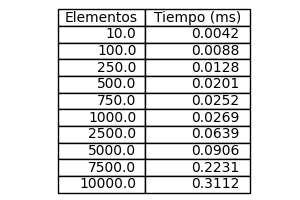
\includegraphics[scale=1]{../tabla-insertion-best.png}  
\end{center}
\begin{center}
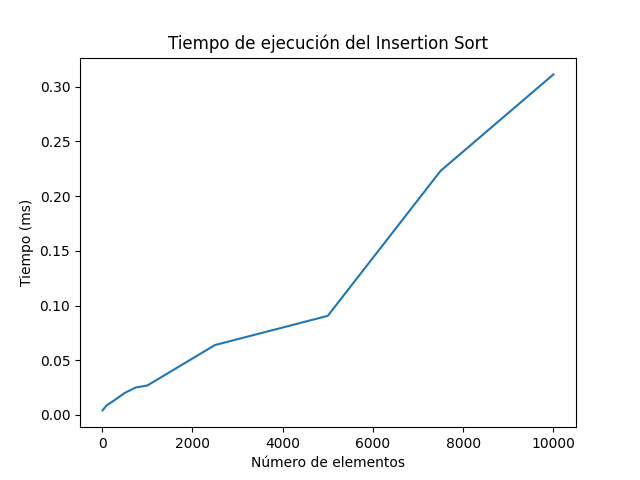
\includegraphics[scale=0.9]{../grafica-insertion-best.png} 
\end{center}
\newpage
Peor de los casos:
\begin{center}
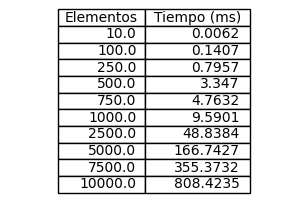
\includegraphics[scale=1]{../tabla-insertion-worst.png}  
\end{center}
\begin{center}
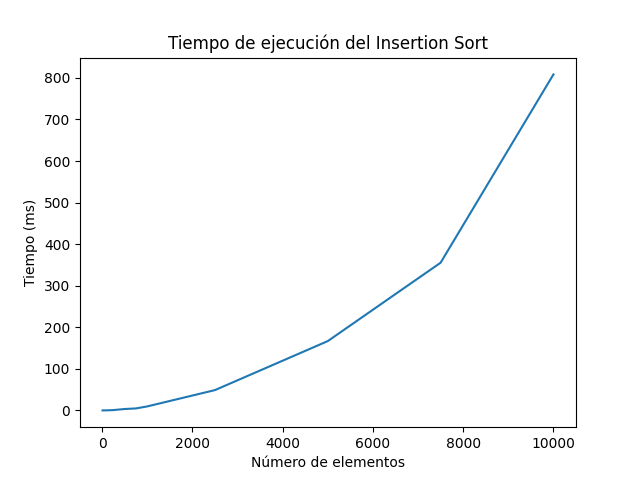
\includegraphics[scale=1]{../grafica-insertion-worst.png} 
\end{center}
\newpage
Caso promedio:
\begin{center}
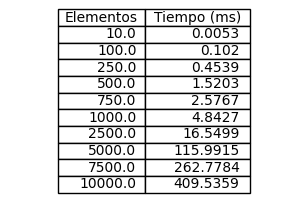
\includegraphics[scale=1]{../tabla-insertion-mean.png}  
\end{center}
\begin{center}
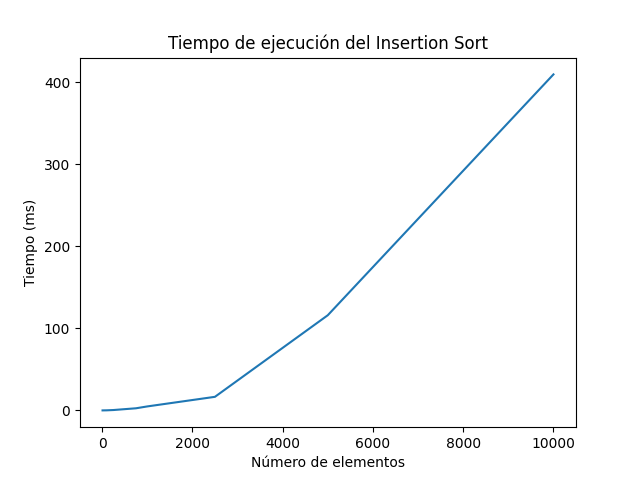
\includegraphics[scale=1]{../grafica-insertion-mean.png} 
\end{center}
\newpage
\subsection*{Selection Sort}
\quad El código del \textit{selection sort} es el siguiente:
\begin{lstlisting}[language=C++]
vector<int> selectionSort(vector<int> arr, int n) {
    int i, j, min_idx;
    for (i = 0; i < n-1; i++) {
        min_idx = i;
        for (j = i+1; j < n; j++) {
            if (arr[j] < arr[min_idx]) {
                min_idx = j;
            }
        }
        swap(arr[min_idx], arr[i]);
    }
    return arr;
}
\end{lstlisting}
Mejor de los casos:
\begin{center}
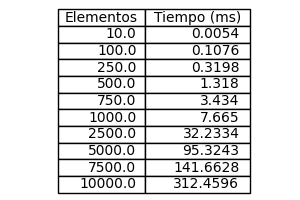
\includegraphics[scale=1]{../tabla-selection-best.png}  
\end{center}
\begin{center}
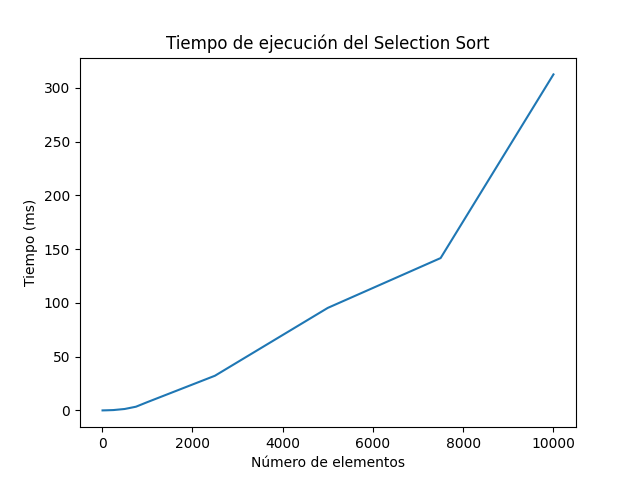
\includegraphics[scale=0.9]{../grafica-selection-best.png} 
\end{center}
\newpage
Peor de los casos:
\begin{center}
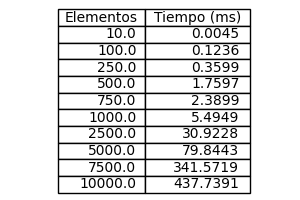
\includegraphics[scale=1]{../tabla-selection-worst.png}  
\end{center}
\begin{center}
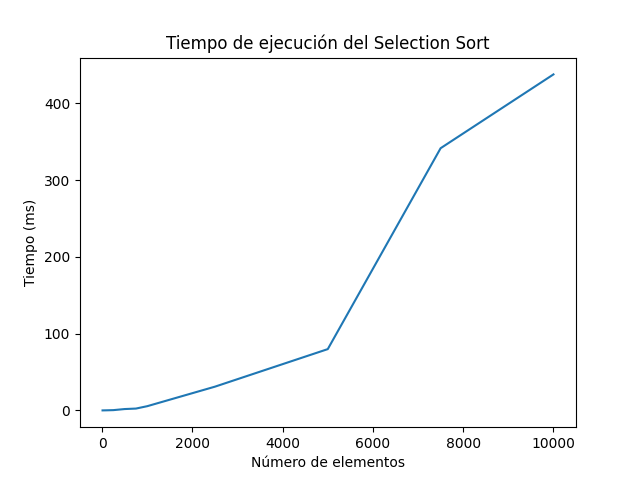
\includegraphics[scale=1]{../grafica-selection-worst.png} 
\end{center}
Caso promedio:
\begin{center}
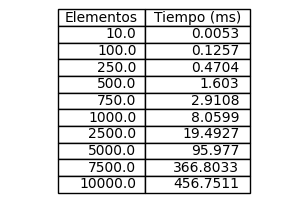
\includegraphics[scale=1]{../tabla-selection-mean.png}  
\end{center}
\begin{center}
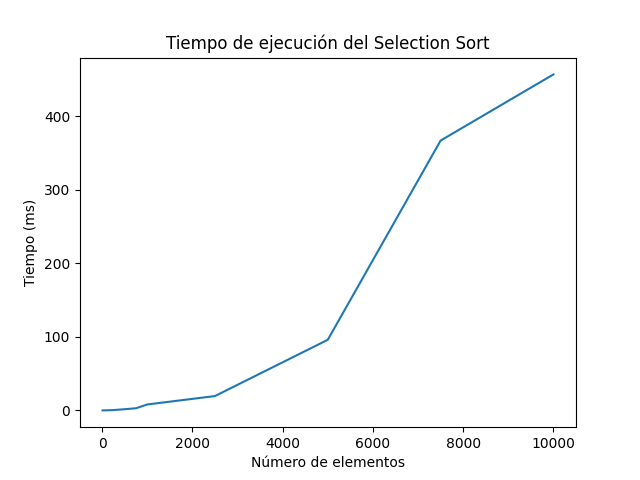
\includegraphics[scale=1]{../grafica-selection-mean.png} 
\end{center}
\newpage
\subsection*{Merge Sort}
\quad El código del \textit{merge sort} es el siguiente:
\begin{lstlisting}[language=C++]
void merge(vector<int> &arr, int left, int middle, int right) {
    int i, j, k;
    int n1 = middle - left + 1;
    int n2 = right - middle;

    vector<int> leftArr(n1);
    vector<int> rightArr(n2);

    for (i = 0; i < n1; i++) {
        leftArr[i] = arr[left + i];
    }
    for (j = 0; j < n2; j++) {
        rightArr[j] = arr[middle + 1 + j];
    }

    i = 0;
    j = 0;
    k = left;

    while (i < n1 && j < n2) {
        if (leftArr[i] <= rightArr[j]) {
            arr[k] = leftArr[i];
            i++;
        } else {
            arr[k] = rightArr[j];
            j++;
        }
        k++;
    }

    while (i < n1) {
        arr[k] = leftArr[i];
        i++;
        k++;
    }

    while (j < n2) {
        arr[k] = rightArr[j];
        j++;
        k++;
    }
}

void mergeSort(vector<int> &arr, int left, int right) {
    if (left < right) {
        int middle = left + (right - left) / 2;

        mergeSort(arr, left, middle);
        mergeSort(arr, middle + 1, right);

        merge(arr, left, middle, right);
    }
}
\end{lstlisting}
\newpage
Mejor de los casos:
\begin{center}
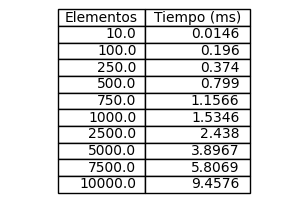
\includegraphics[scale=1]{../tabla-merge-best.png}  
\end{center}
\begin{center}
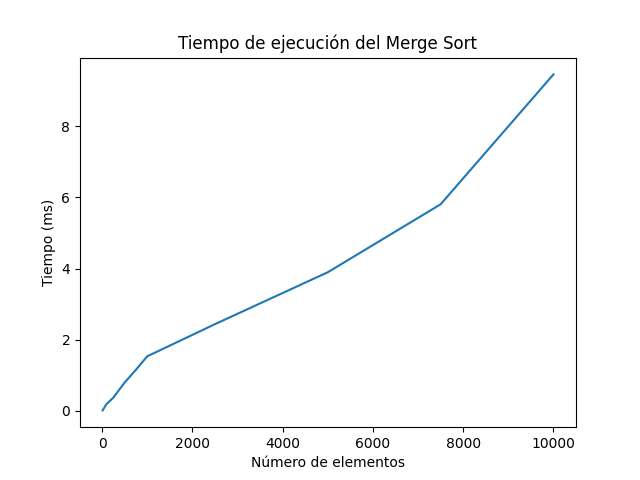
\includegraphics[scale=0.9]{../grafica-merge-best.png} 
\end{center}
Peor de los casos:
\begin{center}
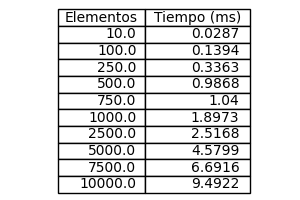
\includegraphics[scale=1]{../tabla-merge-worst.png}  
\end{center}
\begin{center}
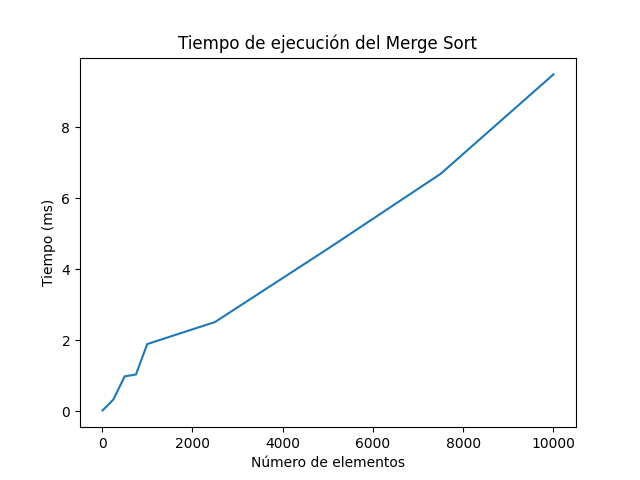
\includegraphics[scale=1]{../grafica-merge-worst.png} 
\end{center}
Caso promedio:
\begin{center}
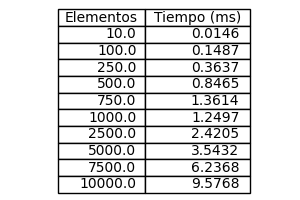
\includegraphics[scale=1]{../tabla-merge-mean.png}  
\end{center}
\begin{center}
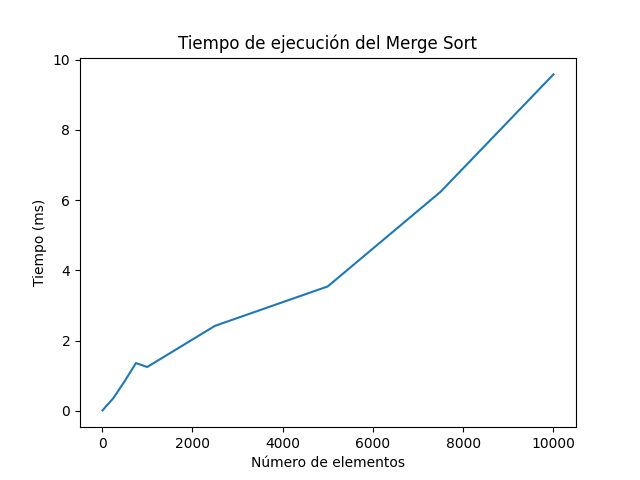
\includegraphics[scale=1]{../grafica-merge-mean.png} 
\end{center}
\newpage
\subsection*{T(n) del Selection Sort}
\quad El algoritmo del \textit{Selection Sort} es el siguiente
\begin{lstlisting}[language=C++]
for i <- 1 to n-1 do
	min j <- i;
	min x <- A[i]
	for j <- i+1 to n do
		if A[j] < min x then
			min j <- i
			min x <- A[j]
	A[min j] <- A[i]
	A[i] <- min x
\end{lstlisting}
\quad El algoritmo ejecuta  dos bucles aninados, el primero o exterior se ejecuta $n$ veces mientras que el interior se ejecuta $n-1$ en la primera iteración del bucle exterior, reduciéndose en uno en cada iteración de este. Así hasta que solo le queda un elemento por ordenar. La función de coste de esta forma se puede expresar como
\begin{equation*}
	T(n)=c_1(n-1)+c_2(n-2)+\cdots +c_{n-1}
\end{equation*}
Donde $c_i$ representa el costo de la operación en la i-ésima iteración del bucle interior, con $n$ la longitud del la lista.
La operación más costosa en el Selection Sort es encontrar el mínimo elemento en la lista, que se realiza en cada iteración del bucle interior. Esta operación tiene un costo de $n$ comparaciones. Por lo tanto, podemos expresar el costo total del Selection Sort como:
\begin{equation*}
T(n) = n-1 + 2(n-2) + 3(n-3) + ... + (n-1)
\end{equation*}
Que es pues la serie aritmética que se expresa como:
\begin{equation*}
	T(n)=\frac{n^2}{2}+\frac{n}{2}
\end{equation*}
\newpage
\subsection*{Funciones f(n)}
\quad Las gráficas de las funciones
\begin{equation*}
	f(n)=log(n)\quad f(n)=n \quad f(n)=nlog(n)
\end{equation*}
\begin{equation*}
	f(n)=n^2\quad f(n)=n^3
\end{equation*}
\begin{center}
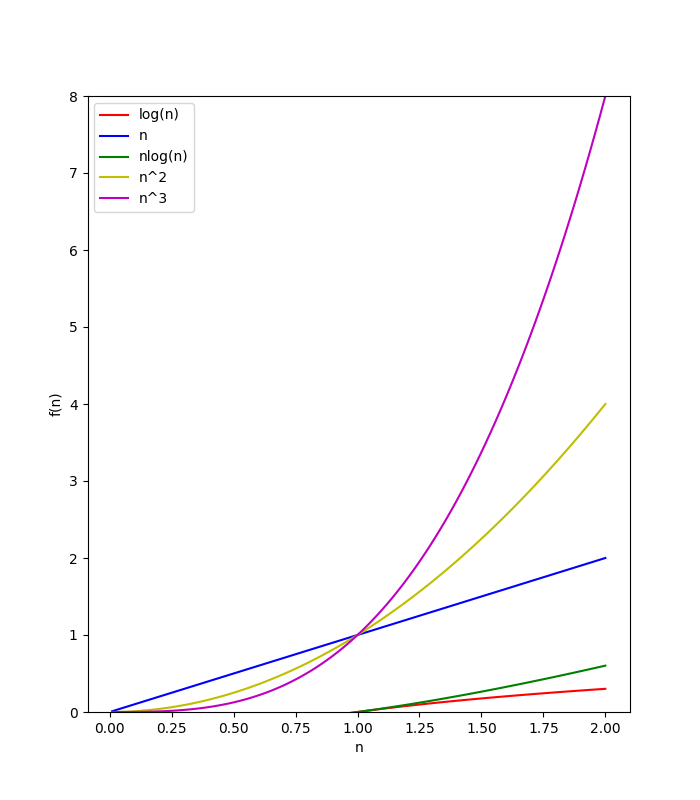
\includegraphics[scale=1]{../grafica-funciones.png} 
\end{center}






\end{document}